\chapter{التقنيات المخبرية الثالثة: ممارسة البحث}\label{ch:b3:lab-techniques-3}

تشتعل قارورة محلول البوتيل ليثيوم إذا لامست قطرةٌ منه الهواء؛ أما \omterm{def:b3:lab-techniques-3:schlenk}{صندوق
القفازات} فيُبقي الأكسجين والماء دون بضعة أجزاء في المليون، بحيث يمكن
وزن مثل هذه المركبات كما يوزن ملح الطعام. وكثيرًا ما يبدأ البحث الكيميائي بإبعاد
الغلاف الجوي، وينتهي بادعاء يجب أن يتمكن الآخرون من
التحقق منه: مركب جديد، تُثبَت بنيته ونقاوته بعدة طرق مستقلة،
وتُسجَّل بياناته وتُنشر بحيث يمكن تكرار العمل. ويجمع هذا
الفصل الأخير ممارسة البحث: التعامل مع \omterm{def:b3:lab-techniques-3:air-sensitive}{المواد الحساسة للهواء}،
وتوصيف مركب جديد، والحكم على نتيجة إحصائيًا،
وتدوين \omterm{def:b3:lab-techniques-3:notebook}{دفتر المختبر} وقراءة الأدبيات العلمية، وتقييم مخاطر
إجراء لم ينفذه أحد من قبل.

\begin{recall}
عالج مجلد السنة الأولى الأخطار، والمخاطر، والرسوم التحذيرية، وعبارات H وP، وصحائف
بيانات السلامة وارتياب القياس بتقييميه من النوعين A وB؛ وعالج مجلد
السنة الثانية الأجواء الخاملة، والمعالجة، ومواد التجفيف، والكروماتوغرافيا الومضية،
ومطيافية الكتلة (HRMS، والكتلة الأحادية النظير)، والرنين المغناطيسي النووي للكربون \babelsublr{$^{13}$C}، ومجالات الثقة،
ومعامل ستيودنت، والمعايرة، والدقة، والصحة، والانحياز، والتكرارية،
والتحقق من صلاحية الطرق، والارتفاع الأديباتي في درجة الحرارة والانفلات الحراري.
وقدّمت \cref{ch:b3:advanced-nmr} و\cref{ch:b3:x-ray-diffraction}
و\cref{ch:b3:electrode-kinetics} الطرق البنيوية
والكهركيميائية.
\end{recall}

\begin{omfigure}
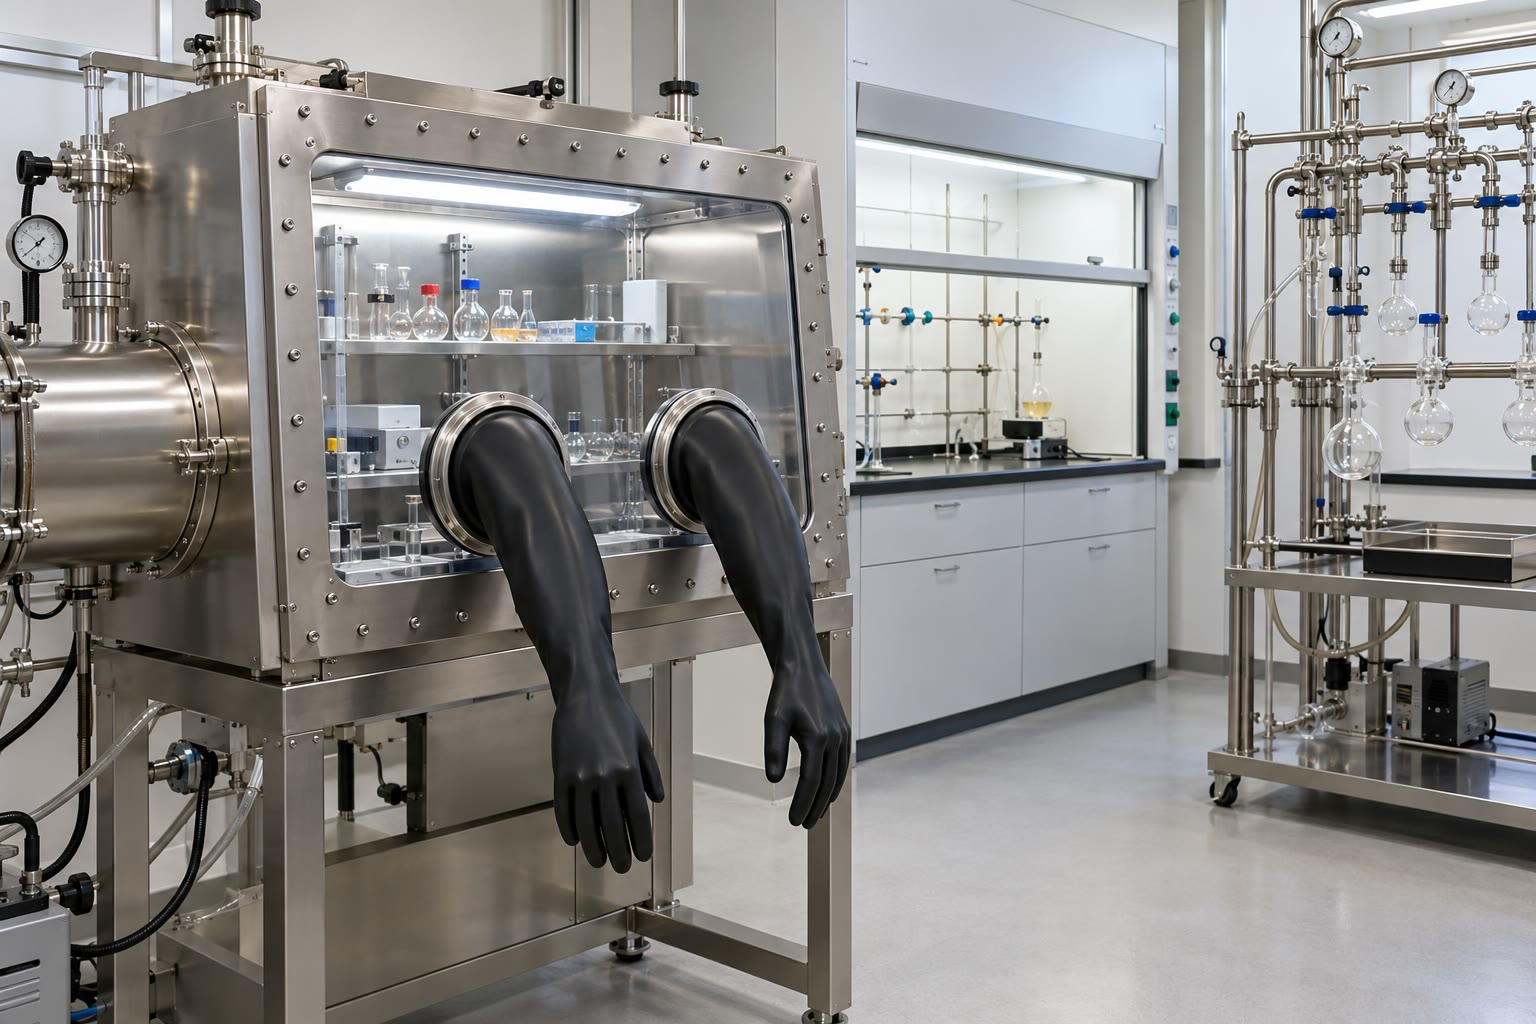
\includegraphics[width=0.58\linewidth]{images/book4/ai/b3-33-glovebox.jpg}

{\small مختبر بحث فيه صندوق قفازات: يُعمل داخل الصندوق الفولاذي المقاوم للصدأ، المملوء
بالنيتروجين الجاف أو بالأرغون، عبر القفازات؛ والأسطوانة على
اليسار هي حجرة العبور لإدخال الأدوات وإخراجها.}
\end{omfigure}

\section{العمل دون هواء}

\begin{definition}[المركبات الحساسة للهواء]\label{def:b3:lab-techniques-3:air-sensitive}
\emph{المركب الحساس للهواء}\index{مركب حساس للهواء} يتفاعل مع
ثنائي الأكسجين أو ماء الهواء، فيتفكك أو يفقد نشاطه. 
و\emph{المادة الذاتية الاشتعال}\index{مادة ذاتية الاشتعال} تشتعل تلقائيًا في
الهواء.
\end{definition}

\begin{definition}[خط شلنك وصندوق القفازات]\label{def:b3:lab-techniques-3:schlenk}
\emph{خط شلنك}\index{خط شلنك} مشعب زجاجي مزدوج، أحد أنبوبيه
متصل بمضخة تفريغ عبر مصيدة باردة، والآخر بمصدر غاز خامل
جاف ينفَّس عبر فقّاعة زيتية، مع صنابير تصل كل مخرج بأي
منهما. و\emph{دورق شلنك}\index{دورق شلنك} له ذراع جانبية بصنبور
لوصله بالخط. و\emph{صندوق القفازات}\index{صندوق القفازات} صندوق محكم الإغلاق
مملوء بغاز خامل يُنقّى باستمرار، ويُعمل داخله عبر
قفازات.
\end{definition}

\begin{omfigure}
\begin{tikzpicture}[font=\scriptsize, >=Stealth]
  % manifolds
  \draw[om glass, line width=1.1pt] (0,3.0) -- (8.0,3.0);
  \draw[om glass, line width=1.1pt] (0,2.5) -- (8.0,2.5);
  \node[anchor=east] at (-1.0,3.0) {\foreignlanguage{arabic}{غاز خامل}};
  \node[anchor=east] at (0,2.5) {\foreignlanguage{arabic}{الفراغ}};
  % taps
  \foreach \x in {2.0,4.0,6.0} {
    \draw[om glass] (\x,3.0) -- (\x,2.5);
    \draw[fill=white] (\x,2.75) circle (0.12);
    \draw (\x-0.1,2.75) -- (\x+0.1,2.75);
    \draw[om glass] (\x,2.5) -- (\x,2.0);
  }
  % flask on the middle tap
  \draw[thick, black!60] (4.0,2.0) -- (4.0,1.6) -- (4.6,1.6);
  \pic[scale=0.5, transform shape] at (5.0,-0.2) {rbflask={0.3}{omDef!20}};
  \draw[om glass] (4.6,1.6) -- (4.9,1.25);
  \node[anchor=west] at (5.4,0.4) {\foreignlanguage{arabic}{دورق شلنك}};
  % bubbler at the gas end
  \pic[scale=0.55, transform shape] at (8.9,1.5) {bubbler};
  \draw[om glass] (8.0,3.0) -- (8.6,3.0) -- (8.6,2.9);
  \node[anchor=west] at (9.4,2.2) {\foreignlanguage{arabic}{فقّاعة زيتية}};
  % trap and pump at the vacuum end
  \draw[om glass] (0.4,2.5) -- (0.4,1.6);
  \draw[om glass, fill=omDef!8] (0.15,1.6) rectangle (0.65,0.4);
  \fill[omDef!25] (0.0,0.2) rectangle (0.8,1.2);
  \node[anchor=north] at (0.4,0.2) {\foreignlanguage{arabic}{مصيدة باردة}};
  \draw[om glass] (0.65,0.9) -- (1.6,0.9);
  \draw[fill=black!15] (1.6,0.6) rectangle (2.6,1.2);
  \node at (2.1,0.9) {\foreignlanguage{arabic}{مضخة}};
  \draw[->, thick] (-0.9,3.0) -- (0,3.0);
\end{tikzpicture}

{\small \omterm{def:b3:lab-techniques-3:schlenk}{خط شلنك}، رسم تخطيطي: مشعب للغاز ومشعب للتفريغ تصل بينهما
صنابير؛ وكل صنبور يصل دورقه إما بالفراغ وإما بالغاز الخامل. وبخار المذيب
المسحوب بالضخ يتكثف في المصيدة الباردة قبل أن يبلغ المضخة؛ ويخرج الغاز
عبر فقّاعة زيتية تمنع الهواء من الرجوع.}
\end{omfigure}

\begin{proposition}[دورات التفريغ--إعادة الملء]\label{prop:b3:lab-techniques-3:purge-cycles}
إذا فُرّغ دورق مملوء بالهواء عند ضغط $p_0$ حتى $p_{\min}$ ثم أُعيد ملؤه
بغاز خامل نقي، وكُرّر ذلك $n$ مرة، فإن جزء الهواء الأصلي المتبقي هو $(p_{\min}/p_0)^n$.
\end{proposition}

\begin{proof}
يترك التفريغ حتى $p_{\min}$ جزءًا $p_{\min}/p_0$ من الغاز، بالتركيب نفسه؛ 
وإعادة الملء بغاز خامل نقي تعيد $p_0$ دون إضافة هواء. فكل دورة تضرب
جزء الهواء في $p_{\min}/p_0$؛ وبعد $n$ دورة يصير $(p_{\min}/p_0)^n$.
\end{proof}

ثلاث دورات حتى \qty{0.1}{mbar} تترك نظريًا $10^{-12}$ من الهواء؛ أما عمليًا فالتسربات، والغاز
الممتز على الزجاج، وانبعاث الغازات من الشحم والحواجز المطاطية تحدد الحد، 
ولهذا تُجفَّف الأدوات الزجاجية في فرن وتُركَّب وهي ساخنة.

\begin{definition}[النقل بالقنية]\label{def:b3:lab-techniques-3:cannula}
\emph{النقل بالقنية}\index{نقل بالقنية} ينقل سائلًا حساسًا للهواء
من وعاء محكم الإغلاق إلى آخر عبر إبرة طويلة ذات طرفين حادين، يدفعه
ضغط زائد صغير من الغاز الخامل في الوعاء الأول.
\end{definition}

\begin{omfigure}
\begin{tikzpicture}[font=\scriptsize, >=Stealth]
  \pic at (0,0) {rbflask={0.35}{omThm!25}};
  \pic at (4.2,0) {rbflask={0.1}{omDef!15}};
  \pic at (0,3.0) {septum};
  \pic at (4.2,3.0) {septum};
  \draw[black!70, line width=0.9pt] (0.05,0.25) -- (0.05,3.5) to[out=90, in=90] (4.15,3.5) -- (4.15,1.6);
  \draw[->, thick, omThm] (1.3,3.95) -- (2.9,3.95) node[midway, above] {\foreignlanguage{arabic}{السائل}};
  \draw[->, thick] (-1.3,3.4) -- (-0.15,3.2) node[pos=0, left] {\foreignlanguage{arabic}{دخول الغاز الخامل بضغط زائد طفيف}};
  \draw[->, thick] (4.35,3.2) -- (5.4,3.6) node[right] {\foreignlanguage{arabic}{تنفيس نحو الفقّاعة}};
  \node[anchor=north] at (0,-0.1) {\foreignlanguage{arabic}{المصدر}};
  \node[anchor=north] at (4.2,-0.1) {\foreignlanguage{arabic}{المستقبِل}};
\end{tikzpicture}

{\small \omterm{def:b3:lab-techniques-3:cannula}{النقل بالقنية}: يغوص الطرف السفلي للقنية في سائل
دورق المصدر؛ والغاز الخامل المُدخل إلى المصدر يدفع السائل عبر
القنية إلى المستقبِل، الذي يُنفَّس عبر إبرة نحو الفقّاعة.}
\end{omfigure}

\begin{method}[النقل بالقنية]\label{met:b3:lab-techniques-3:cannula}
\begin{enumerate}
  \item ضع الدورقين، المغلقين بحاجزين مطاطيين، تحت الغاز الخامل على \omterm{def:b3:lab-techniques-3:schlenk}{خط شلنك}.
  \item اطرد الهواء من القنية بالغاز: أدخل أحد طرفيها في المصدر فوق السائل
        حتى يخرج الغاز من الطرف الآخر، ثم أدخل ذلك الطرف في المستقبِل.
  \item نفّس المستقبِل بإبرة؛ وادفع طرف القنية الذي في المصدر تحت
        سطح السائل: فيدفع الضغط الزائد السائل إلى الجهة الأخرى.
  \item للتوقف، ارفع الطرف فوق السائل؛ واسحب القنية من المستقبِل
        أولًا، واشطفها فورًا بمذيب جاف، ثم بالماء، تحت ساحبة الأبخرة.
\end{enumerate}
\end{method}

\begin{definition}[نزع الغازات بالتجميد--الضخ--الإذابة]\label{def:b3:lab-techniques-3:degassing}
\emph{نزع الغازات بالتجميد--الضخ--الإذابة}\index{نزع الغازات بالتجميد--الضخ--الإذابة} يزيل
الغازات المذابة من سائل بتجميده في النيتروجين السائل، وتفريغ
الحيز فوقه، ثم إغلاق الصنبور وتركه يذوب، فيفلت الغاز المذاب
إلى الفراغ؛ وتُكرَّر الدورة ثلاث مرات.
\end{definition}

تأتي المذيبات الجافة اليوم من أعمدة ألومينا منشَّطة تحت غاز خامل
بدلًا من أجهزة التقطير فوق الصوديوم. ومحاليل المركبات الليثيومية العضوية تفقد قوتها مع
الزمن وتُعاير قبل الاستعمال، مثلًا مقابل كمية موزونة من
حمض ثنائي فينيل الأسيتيك في THF جاف: المكافئ الأول ينزع بروتون الحمض، 
والقطرة الزائدة الأولى تعطي الأنيون الثنائي الأصفر.

\begin{proposition}[عيار مركب ليثيومي عضوي]\label{prop:b3:lab-techniques-3:titre}
إذا احتاجت كتلة $m$ من حمض ثنائي فينيل الأسيتيك (كتلته المولية $M$) إلى حجم $V$ من
محلول مركب ليثيومي عضوي لبلوغ تغير اللون، فإن التركيز هو $c = m/(MV)$.
\end{proposition}

\begin{proof}
حتى نقطة النهاية ينزع كل جزيء من المركب الليثيومي العضوي بروتونًا واحدًا من الحمض؛ 
ويظهر اللون حين يُستهلك الحمض. فالكميتان متساويتان: $cV = m/M$.
\end{proof}

\begin{inthelab}[حجرة العبور في صندوق القفازات]
تدخل الأدوات إلى \omterm{def:b3:lab-techniques-3:schlenk}{صندوق القفازات} عبر حجرة العبور: توضع داخلها، ويُغلق
الباب الخارجي، وتُفرَّغ الحجرة وتُعاد تعبئتها بغاز الصندوق
ثلاث مرات، مع تفريغ أخير طويل للأدوات المسامية، التي تحبس الهواء؛
وعندئذ فقط يُفتح الباب الداخلي من داخل \omterm{def:b3:lab-techniques-3:schlenk}{الصندوق بالقفازات}. ولا تُضخ أبدًا المذيبات
والأوعية المفتوحة التي فيها سوائل متطايرة في حجرة العبور، ولا
يُفتح في الداخل دون إذن أي شيء قد يسمم وحدة التنقية (الثيولات، والمذيبات المهلجنة).
\end{inthelab}

\begin{omfigure}
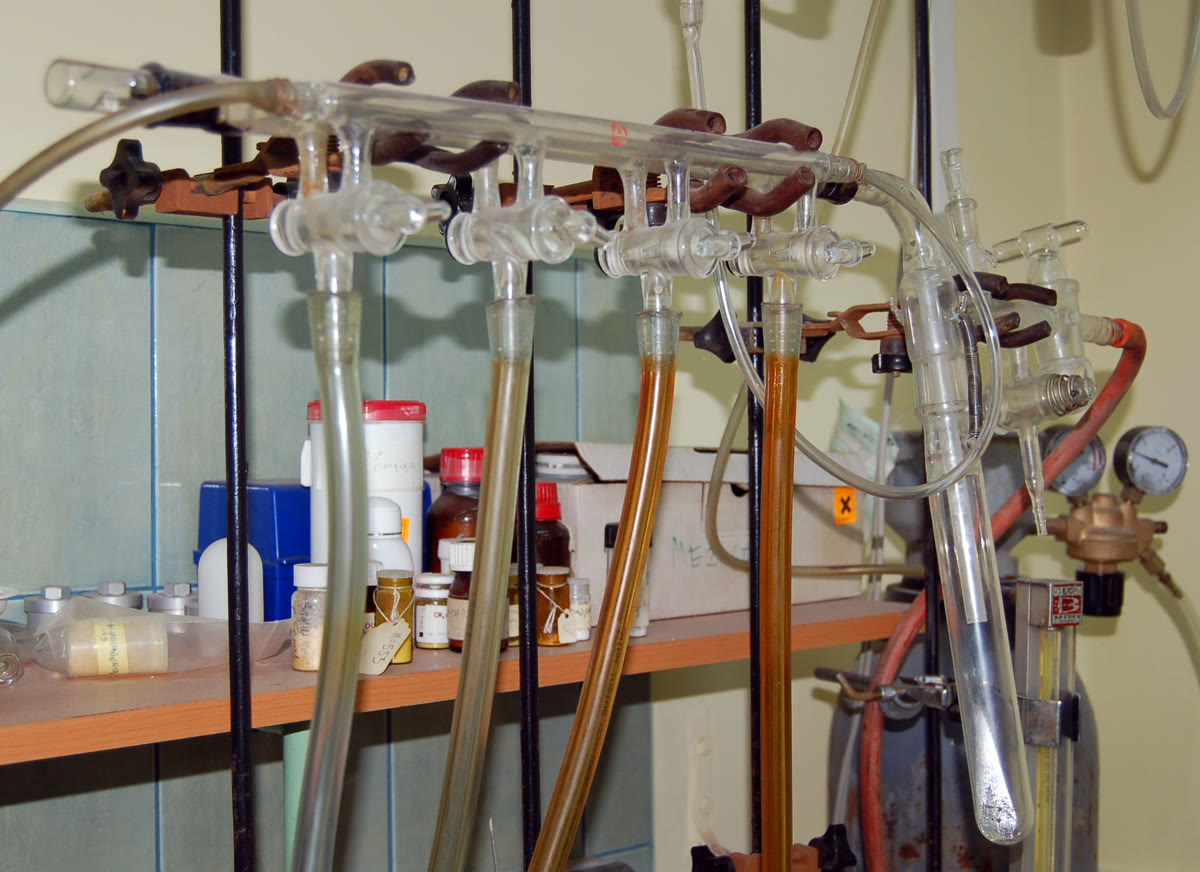
\includegraphics[width=0.46\linewidth]{images/book4/schlenk-line.jpg}

{\small \omterm{def:b3:lab-techniques-3:schlenk}{خط شلنك} قيد الاستعمال: المشعب الزجاجي بصنابيره، والأنابيب الواصلة إلى
الدوارق، ومنظم الغاز. الصورة: Polimerek، CC BY-SA 3.0.}
\end{omfigure}

\section{توصيف مركب جديد}

\begin{method}[توصيف مركب جديد]\label{met:b3:lab-techniques-3:characterise}
\begin{enumerate}
  \item النقاوة: بقعة واحدة في TLC بمحلّين اثنين، وقمة واحدة في HPLC أو GC، ودرجة
        انصهار حادة؛ \omterm{def:b3:lab-techniques-3:qnmr}{والرنين المغناطيسي النووي الكمي} إن لزمت نقاوة كتلية.
  \item الصيغة: HRMS في حدود بضعة أجزاء في المليون من الكتلة المحسوبة، ونمط
        النظائر؛ أو \omterm{def:b3:lab-techniques-3:elemental}{التحليل العنصري}.
  \item البنية: الرنين المغناطيسي النووي للنواتين \babelsublr{$^1$H} و\babelsublr{$^{13}$C} مع تجارب ثنائية البعد للروابط
        (\cref{ch:b3:advanced-nmr})، وتحت الأحمر للمجموعات الوظيفية؛ وبنية بالأشعة السينية لبلورة
        مفردة حين تنمو البلورات (\cref{ch:b3:x-ray-diffraction}).
  \item الكيمياء الفراغية: NOE، وثوابت الاقتران، والدوران الضوئي، \omterm{def:b3:asymmetric-synthesis:ee}{والزيادة المرآوية} بالكروماتوغرافيا
        الكيرالية.
  \item أبلغ عن كل معطى مع ظروفه، وضع الأطياف في \omterm{def:b3:lab-techniques-3:literature}{المعلومات
        الداعمة}.
\end{enumerate}
\end{method}

\begin{omfigure}
\begin{tikzpicture}[font=\scriptsize, >=Stealth,
  box/.style={draw, rounded corners, align=center, fill=omDef!8, inner sep=3pt, minimum height=8mm}]
  \node[box] (a) at (0,0) {\foreignlanguage{arabic}{مركب جديد}\\ \foreignlanguage{arabic}{معزول}};
  \node[box] (b) at (2.85,0) {\foreignlanguage{arabic}{نقي؟}\\ TLC, HPLC\\ \foreignlanguage{arabic}{درجة الانصهار}};
  \node[box] (c) at (5.85,0) {\foreignlanguage{arabic}{الصيغة}\\ HRMS, CHN};
  \node[box] (d) at (8.75,0) {\foreignlanguage{arabic}{البنية}\\ NMR (1D, 2D), IR};
  \node[box] (e) at (8.75,-1.6) {\foreignlanguage{arabic}{أشعة سينية إن وُجدت بلورات،}\\ \foreignlanguage{arabic}{الكيمياء الفراغية}};
  \node[box, fill=omMeth!12] (f) at (5.85,-1.6) {\foreignlanguage{arabic}{متسق؟}\\ \foreignlanguage{arabic}{أبلغ عنه مع}\\ \foreignlanguage{arabic}{البيانات الخام}};
  \node[box, fill=omThm!10] (g) at (2.85,-1.6) {\foreignlanguage{arabic}{أعد التنقية}\\ \foreignlanguage{arabic}{بالكروماتوغرافيا}\\ \foreignlanguage{arabic}{أو بالتبلير}};
  \draw[->, thick] (a) -- (b); \draw[->, thick] (b) -- node[above, inner sep=1pt] {\foreignlanguage{arabic}{نعم}} (c);
  \draw[->, thick] (c) -- (d); \draw[->, thick] (d) -- (e); \draw[->, thick] (e) -- (f);
  \draw[->, thick] (b) -- node[left] {\foreignlanguage{arabic}{لا}} (g); \draw[->, thick] (g.north west) to[bend left=30] (a.south);
\end{tikzpicture}

{\small مسار توصيف مركب جديد: النقاوة أولًا، ثم
الصيغة، ثم البنية؛ وكل ادعاء يستند إلى طريقتين مستقلتين
على الأقل، \omterm{def:b3:lab-techniques-3:notebook}{والبيانات الخام} ترافق التقرير.}
\end{omfigure}

\begin{definition}[التحليل العنصري]\label{def:b3:lab-techniques-3:elemental}
\emph{التحليل العنصري}\index{تحليل عنصري} (التحليل بالاحتراق)
يعيّن النسب المئوية الكتلية للكربون والهيدروجين والنيتروجين والكبريت في
عينة بحرقها في الأكسجين وقياس ثنائي أكسيد الكربون والماء
وثنائي النيتروجين وثنائي أكسيد الكبريت المتكوّنة.
\end{definition}

\begin{proposition}[النسب المئوية الكتلية من صيغة]\label{prop:b3:lab-techniques-3:mass-fractions}
لصيغة $\mathrm{C}_a\mathrm{H}_b\mathrm{N}_c\dots$ كتلتها المولية $M$، تكون النسبة المئوية الكتلية للكربون $100\,aA_r(\mathrm C)/M$، وكذلك
للعناصر الأخرى.
\end{proposition}

\begin{proof}
يحتوي مول واحد من المركب، كتلته $M$، على $a$ مول من ذرات الكربون، كتلتها $aA_r(\mathrm C)$؛
والنسبة، مضروبةً في 100، هي النسبة المئوية الكتلية.
\end{proof}

% ledger: ea:tolerance, hrms:tolerance
تطلب معظم مجلات الكيمياء أن تكون قيم C وH وN المقيسة في حدود 0.4 نقطة
مئوية من القيم المحسوبة، أو قياسًا بمطيافية HRMS في حدود بضعة أجزاء في المليون (5 ppm
لدى بعضها)، دليلًا على التركيب. وقد وجدت دراسة واسعة بين المختبرات أن
العينات النقية نفسها تخطئ المعيار 0.4 بتواتر مدهش، وهذا تذكير بأن
المعيار ليس قانونًا من قوانين الطبيعة.

\begin{proposition}[خطأ HRMS]\label{prop:b3:lab-techniques-3:ppm-error}
خطأ كتلة مقيسة $m_{\mathrm{meas}}$ نسبةً إلى الكتلة المحسوبة $m_{\mathrm{calc}}$ هو
$10^6(m_{\mathrm{meas}} - m_{\mathrm{calc}})/m_{\mathrm{calc}}$ ppm؛ وللأيون تُحسب $m_{\mathrm{calc}}$ من الكتل الأحادية النظير مطروحًا منها (أو مضافًا إليها)
كتلة الإلكترونات المنزوعة (أو المضافة).
\end{proposition}

\begin{proof}[بالتعريف]
خطأ ppm هو الفرق النسبي معبَّرًا عنه بأجزاء في المليون؛ 
وكتلة الأيون تختلف عن كتلة الصيغة المتعادلة بالإلكترونات، \qty{5.486e-4}{u} لكل منها، أي
بضعة أجزاء في المليون عند كتل من بضع مئات.
\end{proof}

\begin{definition}[الرنين المغناطيسي النووي الكمي]\label{def:b3:lab-techniques-3:qnmr}
\emph{الرنين المغناطيسي النووي الكمي}\index{رنين مغناطيسي نووي كمي} (qNMR) يعيّن الكميات أو
النقاوات من تكاملات الإشارات، التي تتناسب مع عدد الأنوية
حين يُسجَّل الطيف باسترخاء كامل بين النبضات، مقابل
معيار داخلي معلوم النقاوة يوزن مع العينة.
\end{definition}

\begin{proposition}[النقاوة بالرنين المغناطيسي النووي الكمي]\label{prop:b3:lab-techniques-3:qnmr}
لعينة كتلتها $m_x$ موزونة مع معيار كتلته $m_s$ ونقاوته $P_s$، مع إشارتين
تكاملاهما $I_x$ و$I_s$ ناتجتين عن $N_x$ و$N_s$ بروتونًا،
\[
  P_x = \frac{I_x}{I_s}\,\frac{N_s}{N_x}\,\frac{M_x}{M_s}\,\frac{m_s}{m_x}\,P_s.
\]
\end{proposition}

\begin{proof}
التكاملات تتناسب مع أعداد البروتونات: $I_x/I_s = (N_xn_x)/(N_sn_s)$. ومع
$n_x = P_xm_x/M_x$ و$n_s = P_sm_s/M_s$، يعطي الحل بالنسبة إلى $P_x$ الصيغة.
\end{proof}

\begin{omfigure}
\begin{tikzpicture}
\begin{axis}[width=0.8\linewidth, height=5.0cm, x dir=reverse, xmin=3.0, xmax=7.0, ymin=-0.05, ymax=1.15, clip=false,
  axis x line=bottom, axis y line=none, xlabel={\babelsublr{$\delta$ / ppm}}, tick label style={font=\scriptsize}, label style={font=\small}]
\addplot[color=omDef, thick] table[x=ppm, y=y] {figdata/out/bachelor-3-qnmr.dat};
\node[font=\scriptsize, anchor=south] at (axis cs:6.09,0.33) {\foreignlanguage{arabic}{المعيار، البروتونات العطرية، 3 H}};
\node[font=\scriptsize, anchor=east] at (axis cs:4.20,0.98) {\foreignlanguage{arabic}{الفيروسين، 10 H}};
\node[font=\scriptsize, anchor=west, align=left] at (axis cs:3.72,0.70) {\foreignlanguage{arabic}{المعيار،}\\ \foreignlanguage{arabic}{$\ce{OCH3}$، 9 H}};
\end{axis}
\end{tikzpicture}

{\small طيف بروتوني مركَّب لعينة فيروسين موزونة مع
1،3،5-ثلاثي ميثوكسي بنزين معيارًا داخليًا (نموذج: 20.0 mg من عينة نقاوتها 98.0\,\%،
و15.0 mg من المعيار). التكاملات تتناسب مع عدد
البروتونات مضروبًا في كمية كل مركب؛ ونسبة الإشارة الأحادية للفيروسين إلى
الإشارة الأحادية العطرية للمعيار تعطي النقاوة.}
\end{omfigure}

\section{إحصاء نتيجة بحثية}

\begin{definition}[اختبارات الدلالة]\label{def:b3:lab-techniques-3:tests}
\emph{اختبار الدلالة}\index{اختبار الدلالة} يقرر ما إذا كانت البيانات
متوافقة مع \emph{فرضية العدم}\index{فرضية العدم}، وهي عادة أنه
لا فرق ولا أثر، عند مستوى مختار من خطر رفضها
خطأً (غالبًا 5\,\%).
\end{definition}

\begin{theorem}[اختبار $t$ لعينتين]\label{thm:b3:lab-techniques-3:t-test}
لمجموعتين من $n_1$ و$n_2$ قياسًا مستقلًا مسحوبة من توزيعات
طبيعية لها الانحراف المعياري نفسه، متوسطاهما $\bar x_1$ و$\bar x_2$ وانحرافهما
المعياري المجمَّع $s_p$، يتبع الإحصاء $t = (\bar x_1 - \bar x_2)/(s_p\sqrt{1/n_1 + 1/n_2})$ قانون ستيودنت بعدد
$n_1 + n_2 - 2$ من درجات الحرية حين يتساوى المتوسطان الحقيقيان. \admitted
\end{theorem}

\begin{proposition}[اختبار $F$]\label{prop:b3:lab-techniques-3:f-test}
بالافتراضات نفسها، تتبع النسبة $F = s_1^2/s_2^2$ بين تبايني عينتين
قانون فيشر بدرجات الحرية $(n_1 - 1, n_2 - 1)$ حين يتساوى التباينان الحقيقيان.
\admitted
\end{proposition}

\begin{method}[هل المردود الجديد أفضل؟]\label{met:b3:lab-techniques-3:compare-means}
\begin{enumerate}
  \item كرّر الإجراءين عدة مرات في الظروف نفسها؛ وسجّل
        كل نتيجة.
  \item قارن التشتتين أولًا (اختبار $F$)؛ فإن تشابها، فاجمعهما:
        $s_p^2 = [(n_1 - 1)s_1^2 + (n_2 - 1)s_2^2]/(n_1 + n_2 - 2)$.
  \item احسب $t$ وقارن $|t|$ بمعامل ستيودنت لعدد $n_1 + n_2 - 2$ من درجات
        الحرية عند المستوى المختار.
  \item إن كانت أكبر: فالفرق دال. وإن كانت أصغر: فالبيانات لا تُظهر فرقًا،
        وهذا لا يثبت أنه غير موجود.
\end{enumerate}
\end{method}

لا تُحذف قيمة مشبوهة أبدًا لأنها مزعجة. فاختبارات القيم الشاذة
تنبّه إليها، لكن القرار يستند إلى \omterm{def:b3:lab-techniques-3:notebook}{دفتر المختبر}: فسبب مسجَّل (خطأ في
الوزن، أو دورق ملوث) يسوّغ رفضها؛ ودونه يُحتفظ بها،
أو تُكرَّر التجربة.

\section{دفتر المختبر وبيانات البحث والأدبيات العلمية}

\begin{definition}[دفتر المختبر والبيانات الخام]\label{def:b3:lab-techniques-3:notebook}
\emph{دفتر المختبر}\index{دفتر المختبر} هو السجل المؤرخ
المتصل غير المعدَّل للتجارب المنجزة، كما أُنجزت. و\emph{البيانات
الخام}\index{بيانات خام} هي السجلات الأصلية للقياسات (ملفات
الأجهزة، وقسائم الوزن، والأطياف) قبل أي معالجة.
\end{definition}

\begin{method}[كتابة مدخل في دفتر المختبر]\label{met:b3:lab-techniques-3:notebook}
\begin{enumerate}
  \item التاريخ، والعنوان، والهدف، وإحالة إلى التجربة السابقة ذات الصلة.
  \item مخطط التفاعل مع الكميات (الكتل، والأحجام، والمولات، والمكافئات)،
        ومصادر الكواشف ودفعاتها، \omterm{def:b3:lab-techniques-3:assessment}{وتقييم المخاطر}.
  \item ما أُنجز وما لوحظ، بالترتيب وفي حينه، بما في ذلك ما
        سار على نحو خاطئ؛ ولا تمحُ أبدًا، بل اشطب بحيث يبقى الأصل مقروءًا.
  \item النتائج: المردودات، وأسماء ملفات \omterm{def:b3:lab-techniques-3:notebook}{البيانات الخام}، واستنتاج؛ ثم وقّع.
\end{enumerate}
\end{method}

\begin{definition}[بيانات FAIR]\label{def:b3:lab-techniques-3:fair}
% ledger: fair:year
\emph{بيانات FAIR}\index{بيانات FAIR} بيانات بحثية قابلة
للإيجاد، وقابلة للوصول، وقابلة للتشغيل البيني، وقابلة لإعادة الاستعمال (والاختصار يجمع الحروف الأولى لهذه الصفات بالإنجليزية): موصوفة ببيانات وصفية غنية 
ومعرِّف دائم، ويمكن استرجاعها ببروتوكولات قياسية، وفي صيغ مفتوحة، مع
ترخيص ومصدر واضحين.
\end{definition}

\begin{definition}[النزاهة البحثية]\label{def:b3:lab-techniques-3:integrity}
\emph{النزاهة البحثية}\index{نزاهة بحثية} هي إجراء البحث والإبلاغ عنه
بأمانة وشفافية. وأخطر انتهاكاتها
\emph{الاختلاق}\index{اختلاق} (اختراع البيانات)، و\emph{التزوير}\index{تزوير}
(تعديل البيانات أو الصور أو الإجراءات) و\emph{الانتحال}\index{انتحال}
(تقديم عمل الآخرين على أنه عمل المرء نفسه).
\end{definition}

\begin{definition}[الأدبيات العلمية]\label{def:b3:lab-techniques-3:literature}
\emph{الأدبيات الأولية}\index{أدبيات أولية} تنشر البحث
الأصلي (المقالات، وبراءات الاختراع، والأطروحات)؛ و\emph{الأدبيات
الثانوية}\index{أدبيات ثانوية} تستعرضه وتنظمه (المقالات الاستعراضية،
والكتب المرجعية، وقواعد البيانات)، والكتب الدراسية تشكّل طبقة ثالثة. و\emph{تحكيم
الأقران}\index{تحكيم الأقران} هو تقييم مخطوطة من خبراء مستقلين
قبل النشر. و\emph{المعلومات الداعمة}\index{معلومات داعمة}
لمقالة ما تحوي التفاصيل التجريبية والبيانات اللازمة
لتكرار العمل والتحقق منه.
\end{definition}

\begin{method}[قراءة إجراء منشور]\label{met:b3:lab-techniques-3:read-paper}
\begin{enumerate}
  \item اقرأ القسم التجريبي \omterm{def:b3:lab-techniques-3:literature}{والمعلومات الداعمة}، لا
        الملخص والمخطط وحدهما.
  \item تحقق من النطاق، والتراكيز، ودرجات الحرارة، والأزمنة، والمعالجة؛ ودوّن
        ما هو ناقص.
  \item تحقق من توصيف النواتج مقابل الطريقة السابقة.
  \item ابحث عن مقالات لاحقة استعملت الإجراء أو صحّحته؛ ونفّذه أولًا على
        نطاق صغير.
\end{enumerate}
\end{method}

تفهرس قواعد بيانات البنى والتفاعلات \omterm{def:b3:lab-techniques-3:literature}{الأدبيات الأولية} بحسب المركب 
وبحسب التحويل، ويُبحث فيها برسم بنية أو تفاعل
بدلًا من الكلمات.

\section{تقييم مخاطر إجراء جديد}

\begin{definition}[تقييم المخاطر]\label{def:b3:lab-techniques-3:assessment}
\emph{تقييم المخاطر}\index{تقييم المخاطر} لإجراء ما يحدد
أخطاره، ويقدّر احتمال الضرر وشدته في الظروف المخطط لها،
ويضع الضوابط التي تخفض المخاطرة إلى مستوى مقبول. 
و\emph{تسلسل الضوابط}\index{تسلسل الضوابط} يرتّبها من الأكثر إلى
الأقل فعالية: الإزالة، والاستبدال، والضوابط الهندسية،
والضوابط الإدارية، ومعدات الوقاية الشخصية.
\end{definition}

\begin{omfigure}
\begin{tikzpicture}[font=\scriptsize]
  \foreach \i/\lab/\col in {0/{\foreignlanguage{arabic}{الإزالة: إزالة الخطر}}/omMeth!40, 1/{\foreignlanguage{arabic}{الاستبدال: كاشف أقل خطرًا}}/omMeth!28, 2/{\foreignlanguage{arabic}{الهندسية: ساحبة الأبخرة، صندوق القفازات، الدروع}}/omDef!22, 3/{\foreignlanguage{arabic}{الإدارية: الإجراءات، التدريب}}/omProp!22, 4/{\foreignlanguage{arabic}{معدات الوقاية الشخصية}}/omThm!22} {
    \pgfmathsetmacro\w{5.4-0.95*\i}
    \fill[\col] ({-\w/2},{-0.75*\i}) -- ({\w/2},{-0.75*\i}) -- ({\w/2-0.475},{-0.75*\i-0.7}) -- ({-\w/2+0.475},{-0.75*\i-0.7}) -- cycle;
    \node[anchor=west] at (3.0,{-0.75*\i-0.35}) {\lab};
    \draw[black!30] ({\w/2-0.2},{-0.75*\i-0.35}) -- (2.95,{-0.75*\i-0.35});
  }
  \node[anchor=east, align=right] at (-2.9,-0.35) {\foreignlanguage{arabic}{الأكثر}\\ \foreignlanguage{arabic}{فعالية}};
  \node[anchor=east, align=right] at (-2.9,-3.35) {\foreignlanguage{arabic}{الأقل}\\ \foreignlanguage{arabic}{فعالية}};
  \draw[->, black!50] (-3.3,-0.85) -- (-3.3,-2.85);
\end{tikzpicture}

{\small \omterm{def:b3:lab-techniques-3:assessment}{تسلسل الضوابط}، في صورة هرم مقلوب: إزالة الخطر أو استبداله
يحمي الجميع، دائمًا؛ أما معدات الوقاية فلا تحمي إلا من
يرتديها، ولا تحميه إلا حين تُرتدى وتكون سليمة.}
\end{omfigure}

\begin{definition}[المركبات المكوِّنة للبيروكسيدات]\label{def:b3:lab-techniques-3:peroxide}
\emph{المركب المكوِّن للبيروكسيدات}\index{مركب مكوِّن للبيروكسيدات} مركب، مثل ثنائي إيثيل
الإيثر، أو رباعي هيدروفوران أو 1،4-ديوكسان، يكوّن ببطء بيروكسيدات متفجرة
مع الهواء أثناء التخزين، ولا سيما بعد الفتح وفي الضوء.
\end{definition}

\begin{method}[تقييم مخاطر إجراء جديد]\label{met:b3:lab-techniques-3:risk-assessment}
\begin{enumerate}
  \item عدّد كل مادة (الكواشف، والمذيبات، والنواتج، والنواتج الثانوية، والغازات
        المنطلقة) مع أخطارها من صحيفة بيانات السلامة.
  \item عدّد العمليات وظروفها (التسخين، والضغط، والنطاق،
        والإخماد، والنفايات)؛ وقدّر الحرارة المنطلقة والارتفاع الأديباتي في درجة الحرارة
        قبل التوسيع إلى نطاق أكبر.
  \item لكل خطر، اختر الضوابط نزولًا في التسلسل؛ وخطط لاستجابة
        الطوارئ (الانسكاب، والحريق، والتعرض) ولمسار النفايات.
  \item اكتبه، واجعل غيرك يراجعه، وأعد النظر فيه بعد التنفيذ الأول.
\end{enumerate}
\end{method}

\begin{safety}{\ghs[0.62cm]{GHS02}\ghs[0.62cm]{GHS05}\ghs[0.62cm]{GHS07}\ghs[0.62cm]{GHS08}}
% ledger: ghs4:BuLi, ghs4:Et2O, ghs4:THF
محاليل البوتيل ليثيوم: ذاتية الاشتعال، وتتفاعل بعنف مع الماء مطلقةً
غازًا قابلًا للاشتعال، وتسبب حروقًا شديدة؛ لا يُتعامل معها إلا تحت غاز خامل، مع دلو
رمل جاف في المتناول ودون ماء قريب. وهيدريد الصوديوم كذلك يطلق
الهيدروجين مع الماء والرطوبة، ويُستعمل في صورة معلَّق في الزيت. وثنائي إيثيل
الإيثر وTHF شديدا الاشتعال \omterm{def:b3:lab-techniques-3:peroxide}{ومكوِّنان للبيروكسيدات}: يُؤرَّخان عند الفتح، ويُختبران بحثًا عن
البيروكسيدات قبل التقطير أو التبخير، ويُتخلص منهما وفق جدول زمني.
\end{safety}

\begin{history}[أدوات شلنك الزجاجية]
صمّم فيلهلم شلنك، وهو يدرس المركبات العضوية للفلزات القلوية والجذور في العقد الثاني من القرن العشرين،
الدوارق والتقنيات التي أتاحت له التعامل معها دون هواء؛ ولا يزال
الخط والدورق يحملان اسمه. وبُنيت أولى صناديق القفازات في
أربعينيات القرن العشرين للمواد المشعة، وسرعان ما تبناها الكيميائيون العاملون على
\omterm{def:b3:lab-techniques-3:air-sensitive}{المركبات الحساسة للهواء}.
\end{history}

\section{تمارين}

\begin{exercise}[$\star$]\label{exo:b3:lab-techniques-3:1}
يُفرَّغ دورق حتى \qty{0.50}{mbar} ويُعاد ملؤه حتى \qty{1013}{mbar} بالأرغون ثلاث مرات. ما جزء
الهواء الأصلي المتبقي نظريًا؟ وما الذي يحد النتيجة فعلًا؟
\end{exercise}

\begin{exercise}[$\star$]\label{exo:b3:lab-techniques-3:2}
عيار محلول بوتيل ليثيوم \qty{1.48}{mol/L}. ما الحجم الذي يجب نقله لتوفير
\qty{20.0}{mmol}؟
\end{exercise}

\begin{exercise}[$\star$]\label{exo:b3:lab-techniques-3:3}
% ledger: mass:C12, mass:H1, mass:Fe56, const4:me.u, hrms:tolerance
احسب الكتلة الدقيقة للكاتيون الجذري للفيروسين $\ce{C10H10Fe+}$ من الكتل الأحادية النظير
(\babelsublr{$^{12}$C}: 12 تمامًا، و\babelsublr{$^1$H}: 1.00782503، و\babelsublr{$^{56}$Fe}: 55.93493633، والإلكترون: \qty{5.486e-4}{u})، وخطأ قيمة مقيسة
186.0129 بأجزاء في المليون.
\end{exercise}

\begin{exercise}[$\star$]\label{exo:b3:lab-techniques-3:4}
صنّف في \omterm{def:b3:lab-techniques-3:literature}{أدبيات أولية} أو ثانوية أو ثالثية: مقالة استعراضية، 
ومقالة في مجلة تنشر تخليقًا جديدًا، وبراءة اختراع، وكتاب مرجعي للثوابت
الفيزيائية، وأطروحة، وكتاب دراسي.
\end{exercise}

\begin{exercise}[$\star\star$]\label{exo:b3:lab-techniques-3:5}
% ledger: ea:tolerance
احسب النسب المئوية الكتلية لعناصر C وH وN في الكافيين، $\ce{C8H10N4O2}$، وقرّر هل تستوفي
القيم المقيسة C 49.31، وH 5.22، وN 28.71\,\% المعيار المعتاد ذا النقاط 0.4.
\end{exercise}

\begin{exercise}[$\star\star$]\label{exo:b3:lab-techniques-3:6}
تحتاج عينة كتلتها \qty{170.0}{mg} من حمض ثنائي فينيل الأسيتيك ($\ce{C14H12O2}$) إلى \qty{0.54}{mL} من محلول بوتيل ليثيوم لبلوغ
نقطة النهاية الصفراء. احسب العيار.
\end{exercise}

\begin{exercise}[$\star\star$]\label{exo:b3:lab-techniques-3:7}
أعطى إجراء قديم مردودات 72 و75 و71 و74 و73\,\%؛ وأعطى إجراء معدَّل 76 و78 و75 و77 
و79\,\%. مع معامل ستيودنت 2.31 لثماني درجات حرية عند 95\,\% (من معطيات التمرين)،
هل التحسن دال؟
\end{exercise}

\begin{exercise}[$\star\star$]\label{exo:b3:lab-techniques-3:8}
تعطي طريقتان ست نتائج لكل منهما، بانحرافين معياريين 0.80 و0.30 (بالوحدات
نفسها). مع قيمة حرجة للإحصاء $F$ تساوي 5.05 لدرجتي الحرية (5، 5) عند 95\,\% (من معطيات
التمرين)، هل تختلف دقتاهما؟
\end{exercise}

\begin{exercise}[$\star\star$]\label{exo:b3:lab-techniques-3:9}
اقترح خطة تخزين واختبار لقوارير THF وثنائي إيثيل
الإيثر في مختبر.
\end{exercise}

\begin{exercise}[$\star\star\star$]\label{exo:b3:lab-techniques-3:10}
يخطط طالب لنزع بروتون كحول بهيدريد الصوديوم في DMF عند 60 °C على
نطاق 50 g. حدّد الأخطار (بما فيها الأخطار الحرارية لهذا المذيب مع
القاعدة) واختر الضوابط نزولًا في التسلسل.
\end{exercise}

\begin{exercise}[$\star\star\star$]\label{exo:b3:lab-techniques-3:11}
انشر الارتيابات المعيارية النسبية للمقادير $I_x$ و$I_s$ (0.50\,\% لكل منهما)، و$m_x$ و$m_s$ (\qty{0.010}{mg} على 20.0
و15.0 mg) و$P_s$ (0.10\,\%) عبر صيغة \omterm{def:b3:lab-techniques-3:qnmr}{الرنين المغناطيسي النووي الكمي}، وأعطِ الارتياب النسبي للمقدار $P_x$.
أي الحدود هو الغالب؟
\end{exercise}

\begin{exercise}[$\star\star\star$]\label{exo:b3:lab-techniques-3:12}
تعطي خمس معايرات 81.2 و82.0 و80.6 و81.5 و89.0 (بالمليلتر). ويعطي اختبار ديكسون
$Q = 0.83$ مقابل قيمة حرجة 0.71 (من معطيات التمرين). هل يجب رفض القيمة
الأخيرة؟ اشرح ما الذي ستتحقق منه أولًا.
\end{exercise}

\section{مسألة: من الدورق إلى الورقة}

\begin{problem}[{مسألة نهاية الأسبوع --- من الدورق إلى الورقة، مركب جديد حساس
للهواء: تخليق الفيروسين تحت النيتروجين، وتوصيفه، 
ونقاوته بالرنين المغناطيسي النووي الكمي، وتقييم مخاطر الإجراء}]
\label{pb:b3:lab-techniques-3:1}
% ledger: aw:C, aw:H, aw:Fe, aw:Cl, aw:O, mass:C12, mass:H1, mass:Fe56, const4:me.u, ghs4:ferrocene
معطيات المسألة. يتفاعل كلوريد الحديد(II) اللامائي (5.00 g) مع
سيكلوبنتاديينيد الصوديوم (مكافئان، من السيكلوبنتاديين وهيدريد الصوديوم في
THF) تحت النيتروجين؛ ويُعزل 5.86 g من الفيروسين البرتقالي، $\ce{Fe(C5H5)2}$. وتُطهَّر الدوارق
بثلاث دورات حتى \qty{0.10}{mbar} انطلاقًا من \qty{1000}{mbar}. ويعطي HRMS القيمة $m/z$ 186.0129 للأيون $\ce{M+}$؛ ويعطي \omterm{def:b3:lab-techniques-3:elemental}{التحليل
العنصري} C 64.41، وH 5.47\,\%. وفي $\ce{CDCl3}$ يعطي الفيروسين إشارة أحادية عند 4.16 ppm (10 H). ومن أجل qNMR،
يعطي 20.0 mg من العينة و15.0 mg من 1،3،5-ثلاثي ميثوكسي بنزين (نقاوته 99.9\,\%، وإشارته الأحادية
العطرية عند 6.09 ppm، 3 H) النسبة $I_x/I_s = 3.942$، مع ارتيابات معيارية نسبية قدرها 0.50\,\% لكل
تكامل، و\qty{0.010}{mg} لكل كتلة و0.10\,\% للنقاوة $P_s$.

\medskip\noindent\textbf{الجزء الأول --- التخليق تحت النيتروجين.}
\begin{enumerate}
  \item اكتب معادلة التخليق.
  \item لماذا يجب إجراء التفاعل دون هواء؟
  \item احسب الكتلة النظرية للفيروسين والمردود.
  \item احسب جزء الهواء المتبقي بعد دورات التطهير الثلاث.
  \item كيف يُحصل على السيكلوبنتاديين من ثنائيه، ولماذا يجب استعماله فورًا؟
  \item لماذا يُضاف هيدريد الصوديوم على دفعات؟
\end{enumerate}

\medskip\noindent\textbf{الجزء الثاني --- التوصيف.}
\begin{enumerate}[resume]
  \item احسب الكتلة الدقيقة للأيون $\ce{M+}$ وخطأ القياس بأجزاء في المليون.
  \item احسب النسبتين المئويتين الكتليتين للكربون والهيدروجين وقارنهما بالتحليل.
  \item لماذا يُظهر الفيروسين إشارة واحدة للنواة \babelsublr{$^1$H}؟
  \item ماذا سيُظهر طيف الرنين المغناطيسي النووي للنواة \babelsublr{$^{13}$C}؟
  \item أي طريقة إضافية تثبت البنية الشطيرية؟
  \item هل الفيروسين نفسه حساس للهواء بعد صنعه؟ قارنه بسلائفه.
\end{enumerate}

\medskip\noindent\textbf{الجزء الثالث --- النقاوة \omterm{def:b3:lab-techniques-3:qnmr}{بالرنين المغناطيسي النووي الكمي}.}
\begin{enumerate}[resume]
  \item لماذا يُختار 1،3،5-ثلاثي ميثوكسي بنزين معيارًا هنا؟
  \item ما الذي يجب أن يضمنه تسجيل الطيف لتكون التكاملات كمية؟
  \item احسب الكتلتين الموليتين للفيروسين وللمعيار.
  \item احسب نقاوة العينة.
  \item احسب ارتيابها المعياري النسبي والمطلق.
  \item هل \omterm{def:b3:lab-techniques-3:elemental}{التحليل العنصري} متسق مع هذه النقاوة؟
\end{enumerate}

\medskip\noindent\textbf{الجزء الرابع --- المخاطر وقياس أخير.}
\begin{enumerate}[resume]
  \item عدّد أخطار الإجراء.
  \item اختر ضوابط لهيدريد الصوديوم وللمذيب THF.
  \item كيف يجب إتلاف الفائض من هيدريد الصوديوم في النهاية؟
  \item ماذا يُظهر \omterm{def:b3:electrode-kinetics:cv}{الفولتاموغرام} الدوري للفيروسين، ولماذا يُستعمل الفيروسين
        مرجعًا في الكيمياء الكهربائية؟
  \item ما الذي يجب أن يحتويه مدخل \omterm{def:b3:lab-techniques-3:notebook}{دفتر المختبر} \omterm{def:b3:lab-techniques-3:literature}{والمعلومات الداعمة}؟
  \item لماذا ينبغي أرشفة الأطياف الخام في صيغة مفتوحة؟
  \item اذكر النتيجة: نقاوة عينة الفيروسين \omterm{def:b3:lab-techniques-3:qnmr}{بالرنين المغناطيسي النووي الكمي} مع ارتيابها
        المعياري.
\end{enumerate}
\end{problem}
